\documentclass[10pt]{article}
\usepackage{tmlr}
% For camera-ready: \usepackage[accepted]{tmlr}
% For preprint: \usepackage[preprint]{tmlr}

%%%%% NEW MATH DEFINITIONS %%%%%

\usepackage{amsmath,amsfonts,bm}

% Mark sections of captions for referring to divisions of figures
\newcommand{\figleft}{{\em (Left)}}
\newcommand{\figcenter}{{\em (Center)}}
\newcommand{\figright}{{\em (Right)}}
\newcommand{\figtop}{{\em (Top)}}
\newcommand{\figbottom}{{\em (Bottom)}}
\newcommand{\captiona}{{\em (a)}}
\newcommand{\captionb}{{\em (b)}}
\newcommand{\captionc}{{\em (c)}}
\newcommand{\captiond}{{\em (d)}}

% Highlight a newly defined term
\newcommand{\newterm}[1]{{\bf #1}}


% Figure reference, lower-case.
\def\figref#1{figure~\ref{#1}}
% Figure reference, capital. For start of sentence
\def\Figref#1{Figure~\ref{#1}}
\def\twofigref#1#2{figures \ref{#1} and \ref{#2}}
\def\quadfigref#1#2#3#4{figures \ref{#1}, \ref{#2}, \ref{#3} and \ref{#4}}
% Section reference, lower-case.
\def\secref#1{section~\ref{#1}}
% Section reference, capital.
\def\Secref#1{Section~\ref{#1}}
% Reference to two sections.
\def\twosecrefs#1#2{sections \ref{#1} and \ref{#2}}
% Reference to three sections.
\def\secrefs#1#2#3{sections \ref{#1}, \ref{#2} and \ref{#3}}
% Reference to an equation, lower-case.
\def\eqref#1{equation~\ref{#1}}
% Reference to an equation, upper case
\def\Eqref#1{Equation~\ref{#1}}
% A raw reference to an equation---avoid using if possible
\def\plaineqref#1{\ref{#1}}
% Reference to a chapter, lower-case.
\def\chapref#1{chapter~\ref{#1}}
% Reference to an equation, upper case.
\def\Chapref#1{Chapter~\ref{#1}}
% Reference to a range of chapters
\def\rangechapref#1#2{chapters\ref{#1}--\ref{#2}}
% Reference to an algorithm, lower-case.
\def\algref#1{algorithm~\ref{#1}}
% Reference to an algorithm, upper case.
\def\Algref#1{Algorithm~\ref{#1}}
\def\twoalgref#1#2{algorithms \ref{#1} and \ref{#2}}
\def\Twoalgref#1#2{Algorithms \ref{#1} and \ref{#2}}
% Reference to a part, lower case
\def\partref#1{part~\ref{#1}}
% Reference to a part, upper case
\def\Partref#1{Part~\ref{#1}}
\def\twopartref#1#2{parts \ref{#1} and \ref{#2}}

\def\ceil#1{\lceil #1 \rceil}
\def\floor#1{\lfloor #1 \rfloor}
\def\1{\bm{1}}
\newcommand{\train}{\mathcal{D}}
\newcommand{\valid}{\mathcal{D_{\mathrm{valid}}}}
\newcommand{\test}{\mathcal{D_{\mathrm{test}}}}

\def\eps{{\epsilon}}


% Random variables
\def\reta{{\textnormal{$\eta$}}}
\def\ra{{\textnormal{a}}}
\def\rb{{\textnormal{b}}}
\def\rc{{\textnormal{c}}}
\def\rd{{\textnormal{d}}}
\def\re{{\textnormal{e}}}
\def\rf{{\textnormal{f}}}
\def\rg{{\textnormal{g}}}
\def\rh{{\textnormal{h}}}
\def\ri{{\textnormal{i}}}
\def\rj{{\textnormal{j}}}
\def\rk{{\textnormal{k}}}
\def\rl{{\textnormal{l}}}
% rm is already a command, just don't name any random variables m
\def\rn{{\textnormal{n}}}
\def\ro{{\textnormal{o}}}
\def\rp{{\textnormal{p}}}
\def\rq{{\textnormal{q}}}
\def\rr{{\textnormal{r}}}
\def\rs{{\textnormal{s}}}
\def\rt{{\textnormal{t}}}
\def\ru{{\textnormal{u}}}
\def\rv{{\textnormal{v}}}
\def\rw{{\textnormal{w}}}
\def\rx{{\textnormal{x}}}
\def\ry{{\textnormal{y}}}
\def\rz{{\textnormal{z}}}

% Random vectors
\def\rvepsilon{{\mathbf{\epsilon}}}
\def\rvtheta{{\mathbf{\theta}}}
\def\rva{{\mathbf{a}}}
\def\rvb{{\mathbf{b}}}
\def\rvc{{\mathbf{c}}}
\def\rvd{{\mathbf{d}}}
\def\rve{{\mathbf{e}}}
\def\rvf{{\mathbf{f}}}
\def\rvg{{\mathbf{g}}}
\def\rvh{{\mathbf{h}}}
\def\rvu{{\mathbf{i}}}
\def\rvj{{\mathbf{j}}}
\def\rvk{{\mathbf{k}}}
\def\rvl{{\mathbf{l}}}
\def\rvm{{\mathbf{m}}}
\def\rvn{{\mathbf{n}}}
\def\rvo{{\mathbf{o}}}
\def\rvp{{\mathbf{p}}}
\def\rvq{{\mathbf{q}}}
\def\rvr{{\mathbf{r}}}
\def\rvs{{\mathbf{s}}}
\def\rvt{{\mathbf{t}}}
\def\rvu{{\mathbf{u}}}
\def\rvv{{\mathbf{v}}}
\def\rvw{{\mathbf{w}}}
\def\rvx{{\mathbf{x}}}
\def\rvy{{\mathbf{y}}}
\def\rvz{{\mathbf{z}}}

% Elements of random vectors
\def\erva{{\textnormal{a}}}
\def\ervb{{\textnormal{b}}}
\def\ervc{{\textnormal{c}}}
\def\ervd{{\textnormal{d}}}
\def\erve{{\textnormal{e}}}
\def\ervf{{\textnormal{f}}}
\def\ervg{{\textnormal{g}}}
\def\ervh{{\textnormal{h}}}
\def\ervi{{\textnormal{i}}}
\def\ervj{{\textnormal{j}}}
\def\ervk{{\textnormal{k}}}
\def\ervl{{\textnormal{l}}}
\def\ervm{{\textnormal{m}}}
\def\ervn{{\textnormal{n}}}
\def\ervo{{\textnormal{o}}}
\def\ervp{{\textnormal{p}}}
\def\ervq{{\textnormal{q}}}
\def\ervr{{\textnormal{r}}}
\def\ervs{{\textnormal{s}}}
\def\ervt{{\textnormal{t}}}
\def\ervu{{\textnormal{u}}}
\def\ervv{{\textnormal{v}}}
\def\ervw{{\textnormal{w}}}
\def\ervx{{\textnormal{x}}}
\def\ervy{{\textnormal{y}}}
\def\ervz{{\textnormal{z}}}

% Random matrices
\def\rmA{{\mathbf{A}}}
\def\rmB{{\mathbf{B}}}
\def\rmC{{\mathbf{C}}}
\def\rmD{{\mathbf{D}}}
\def\rmE{{\mathbf{E}}}
\def\rmF{{\mathbf{F}}}
\def\rmG{{\mathbf{G}}}
\def\rmH{{\mathbf{H}}}
\def\rmI{{\mathbf{I}}}
\def\rmJ{{\mathbf{J}}}
\def\rmK{{\mathbf{K}}}
\def\rmL{{\mathbf{L}}}
\def\rmM{{\mathbf{M}}}
\def\rmN{{\mathbf{N}}}
\def\rmO{{\mathbf{O}}}
\def\rmP{{\mathbf{P}}}
\def\rmQ{{\mathbf{Q}}}
\def\rmR{{\mathbf{R}}}
\def\rmS{{\mathbf{S}}}
\def\rmT{{\mathbf{T}}}
\def\rmU{{\mathbf{U}}}
\def\rmV{{\mathbf{V}}}
\def\rmW{{\mathbf{W}}}
\def\rmX{{\mathbf{X}}}
\def\rmY{{\mathbf{Y}}}
\def\rmZ{{\mathbf{Z}}}

% Elements of random matrices
\def\ermA{{\textnormal{A}}}
\def\ermB{{\textnormal{B}}}
\def\ermC{{\textnormal{C}}}
\def\ermD{{\textnormal{D}}}
\def\ermE{{\textnormal{E}}}
\def\ermF{{\textnormal{F}}}
\def\ermG{{\textnormal{G}}}
\def\ermH{{\textnormal{H}}}
\def\ermI{{\textnormal{I}}}
\def\ermJ{{\textnormal{J}}}
\def\ermK{{\textnormal{K}}}
\def\ermL{{\textnormal{L}}}
\def\ermM{{\textnormal{M}}}
\def\ermN{{\textnormal{N}}}
\def\ermO{{\textnormal{O}}}
\def\ermP{{\textnormal{P}}}
\def\ermQ{{\textnormal{Q}}}
\def\ermR{{\textnormal{R}}}
\def\ermS{{\textnormal{S}}}
\def\ermT{{\textnormal{T}}}
\def\ermU{{\textnormal{U}}}
\def\ermV{{\textnormal{V}}}
\def\ermW{{\textnormal{W}}}
\def\ermX{{\textnormal{X}}}
\def\ermY{{\textnormal{Y}}}
\def\ermZ{{\textnormal{Z}}}

% Vectors
\def\vzero{{\bm{0}}}
\def\vone{{\bm{1}}}
\def\vmu{{\bm{\mu}}}
\def\vtheta{{\bm{\theta}}}
\def\va{{\bm{a}}}
\def\vb{{\bm{b}}}
\def\vc{{\bm{c}}}
\def\vd{{\bm{d}}}
\def\ve{{\bm{e}}}
\def\vf{{\bm{f}}}
\def\vg{{\bm{g}}}
\def\vh{{\bm{h}}}
\def\vi{{\bm{i}}}
\def\vj{{\bm{j}}}
\def\vk{{\bm{k}}}
\def\vl{{\bm{l}}}
\def\vm{{\bm{m}}}
\def\vn{{\bm{n}}}
\def\vo{{\bm{o}}}
\def\vp{{\bm{p}}}
\def\vq{{\bm{q}}}
\def\vr{{\bm{r}}}
\def\vs{{\bm{s}}}
\def\vt{{\bm{t}}}
\def\vu{{\bm{u}}}
\def\vv{{\bm{v}}}
\def\vw{{\bm{w}}}
\def\vx{{\bm{x}}}
\def\vy{{\bm{y}}}
\def\vz{{\bm{z}}}

% Elements of vectors
\def\evalpha{{\alpha}}
\def\evbeta{{\beta}}
\def\evepsilon{{\epsilon}}
\def\evlambda{{\lambda}}
\def\evomega{{\omega}}
\def\evmu{{\mu}}
\def\evpsi{{\psi}}
\def\evsigma{{\sigma}}
\def\evtheta{{\theta}}
\def\eva{{a}}
\def\evb{{b}}
\def\evc{{c}}
\def\evd{{d}}
\def\eve{{e}}
\def\evf{{f}}
\def\evg{{g}}
\def\evh{{h}}
\def\evi{{i}}
\def\evj{{j}}
\def\evk{{k}}
\def\evl{{l}}
\def\evm{{m}}
\def\evn{{n}}
\def\evo{{o}}
\def\evp{{p}}
\def\evq{{q}}
\def\evr{{r}}
\def\evs{{s}}
\def\evt{{t}}
\def\evu{{u}}
\def\evv{{v}}
\def\evw{{w}}
\def\evx{{x}}
\def\evy{{y}}
\def\evz{{z}}

% Matrix
\def\mA{{\bm{A}}}
\def\mB{{\bm{B}}}
\def\mC{{\bm{C}}}
\def\mD{{\bm{D}}}
\def\mE{{\bm{E}}}
\def\mF{{\bm{F}}}
\def\mG{{\bm{G}}}
\def\mH{{\bm{H}}}
\def\mI{{\bm{I}}}
\def\mJ{{\bm{J}}}
\def\mK{{\bm{K}}}
\def\mL{{\bm{L}}}
\def\mM{{\bm{M}}}
\def\mN{{\bm{N}}}
\def\mO{{\bm{O}}}
\def\mP{{\bm{P}}}
\def\mQ{{\bm{Q}}}
\def\mR{{\bm{R}}}
\def\mS{{\bm{S}}}
\def\mT{{\bm{T}}}
\def\mU{{\bm{U}}}
\def\mV{{\bm{V}}}
\def\mW{{\bm{W}}}
\def\mX{{\bm{X}}}
\def\mY{{\bm{Y}}}
\def\mZ{{\bm{Z}}}
\def\mBeta{{\bm{\beta}}}
\def\mPhi{{\bm{\Phi}}}
\def\mLambda{{\bm{\Lambda}}}
\def\mSigma{{\bm{\Sigma}}}

% Tensor
\DeclareMathAlphabet{\mathsfit}{\encodingdefault}{\sfdefault}{m}{sl}
\SetMathAlphabet{\mathsfit}{bold}{\encodingdefault}{\sfdefault}{bx}{n}
\newcommand{\tens}[1]{\bm{\mathsfit{#1}}}
\def\tA{{\tens{A}}}
\def\tB{{\tens{B}}}
\def\tC{{\tens{C}}}
\def\tD{{\tens{D}}}
\def\tE{{\tens{E}}}
\def\tF{{\tens{F}}}
\def\tG{{\tens{G}}}
\def\tH{{\tens{H}}}
\def\tI{{\tens{I}}}
\def\tJ{{\tens{J}}}
\def\tK{{\tens{K}}}
\def\tL{{\tens{L}}}
\def\tM{{\tens{M}}}
\def\tN{{\tens{N}}}
\def\tO{{\tens{O}}}
\def\tP{{\tens{P}}}
\def\tQ{{\tens{Q}}}
\def\tR{{\tens{R}}}
\def\tS{{\tens{S}}}
\def\tT{{\tens{T}}}
\def\tU{{\tens{U}}}
\def\tV{{\tens{V}}}
\def\tW{{\tens{W}}}
\def\tX{{\tens{X}}}
\def\tY{{\tens{Y}}}
\def\tZ{{\tens{Z}}}


% Graph
\def\gA{{\mathcal{A}}}
\def\gB{{\mathcal{B}}}
\def\gC{{\mathcal{C}}}
\def\gD{{\mathcal{D}}}
\def\gE{{\mathcal{E}}}
\def\gF{{\mathcal{F}}}
\def\gG{{\mathcal{G}}}
\def\gH{{\mathcal{H}}}
\def\gI{{\mathcal{I}}}
\def\gJ{{\mathcal{J}}}
\def\gK{{\mathcal{K}}}
\def\gL{{\mathcal{L}}}
\def\gM{{\mathcal{M}}}
\def\gN{{\mathcal{N}}}
\def\gO{{\mathcal{O}}}
\def\gP{{\mathcal{P}}}
\def\gQ{{\mathcal{Q}}}
\def\gR{{\mathcal{R}}}
\def\gS{{\mathcal{S}}}
\def\gT{{\mathcal{T}}}
\def\gU{{\mathcal{U}}}
\def\gV{{\mathcal{V}}}
\def\gW{{\mathcal{W}}}
\def\gX{{\mathcal{X}}}
\def\gY{{\mathcal{Y}}}
\def\gZ{{\mathcal{Z}}}

% Sets
\def\sA{{\mathbb{A}}}
\def\sB{{\mathbb{B}}}
\def\sC{{\mathbb{C}}}
\def\sD{{\mathbb{D}}}
% Don't use a set called E, because this would be the same as our symbol
% for expectation.
\def\sF{{\mathbb{F}}}
\def\sG{{\mathbb{G}}}
\def\sH{{\mathbb{H}}}
\def\sI{{\mathbb{I}}}
\def\sJ{{\mathbb{J}}}
\def\sK{{\mathbb{K}}}
\def\sL{{\mathbb{L}}}
\def\sM{{\mathbb{M}}}
\def\sN{{\mathbb{N}}}
\def\sO{{\mathbb{O}}}
\def\sP{{\mathbb{P}}}
\def\sQ{{\mathbb{Q}}}
\def\sR{{\mathbb{R}}}
\def\sS{{\mathbb{S}}}
\def\sT{{\mathbb{T}}}
\def\sU{{\mathbb{U}}}
\def\sV{{\mathbb{V}}}
\def\sW{{\mathbb{W}}}
\def\sX{{\mathbb{X}}}
\def\sY{{\mathbb{Y}}}
\def\sZ{{\mathbb{Z}}}

% Entries of a matrix
\def\emLambda{{\Lambda}}
\def\emA{{A}}
\def\emB{{B}}
\def\emC{{C}}
\def\emD{{D}}
\def\emE{{E}}
\def\emF{{F}}
\def\emG{{G}}
\def\emH{{H}}
\def\emI{{I}}
\def\emJ{{J}}
\def\emK{{K}}
\def\emL{{L}}
\def\emM{{M}}
\def\emN{{N}}
\def\emO{{O}}
\def\emP{{P}}
\def\emQ{{Q}}
\def\emR{{R}}
\def\emS{{S}}
\def\emT{{T}}
\def\emU{{U}}
\def\emV{{V}}
\def\emW{{W}}
\def\emX{{X}}
\def\emY{{Y}}
\def\emZ{{Z}}
\def\emSigma{{\Sigma}}

% entries of a tensor
% Same font as tensor, without \bm wrapper
\newcommand{\etens}[1]{\mathsfit{#1}}
\def\etLambda{{\etens{\Lambda}}}
\def\etA{{\etens{A}}}
\def\etB{{\etens{B}}}
\def\etC{{\etens{C}}}
\def\etD{{\etens{D}}}
\def\etE{{\etens{E}}}
\def\etF{{\etens{F}}}
\def\etG{{\etens{G}}}
\def\etH{{\etens{H}}}
\def\etI{{\etens{I}}}
\def\etJ{{\etens{J}}}
\def\etK{{\etens{K}}}
\def\etL{{\etens{L}}}
\def\etM{{\etens{M}}}
\def\etN{{\etens{N}}}
\def\etO{{\etens{O}}}
\def\etP{{\etens{P}}}
\def\etQ{{\etens{Q}}}
\def\etR{{\etens{R}}}
\def\etS{{\etens{S}}}
\def\etT{{\etens{T}}}
\def\etU{{\etens{U}}}
\def\etV{{\etens{V}}}
\def\etW{{\etens{W}}}
\def\etX{{\etens{X}}}
\def\etY{{\etens{Y}}}
\def\etZ{{\etens{Z}}}

% The true underlying data generating distribution
\newcommand{\pdata}{p_{\rm{data}}}
% The empirical distribution defined by the training set
\newcommand{\ptrain}{\hat{p}_{\rm{data}}}
\newcommand{\Ptrain}{\hat{P}_{\rm{data}}}
% The model distribution
\newcommand{\pmodel}{p_{\rm{model}}}
\newcommand{\Pmodel}{P_{\rm{model}}}
\newcommand{\ptildemodel}{\tilde{p}_{\rm{model}}}
% Stochastic autoencoder distributions
\newcommand{\pencode}{p_{\rm{encoder}}}
\newcommand{\pdecode}{p_{\rm{decoder}}}
\newcommand{\precons}{p_{\rm{reconstruct}}}

\newcommand{\laplace}{\mathrm{Laplace}} % Laplace distribution

\newcommand{\E}{\mathbb{E}}
\newcommand{\Ls}{\mathcal{L}}
\newcommand{\R}{\mathbb{R}}
\newcommand{\emp}{\tilde{p}}
\newcommand{\lr}{\alpha}
\newcommand{\reg}{\lambda}
\newcommand{\rect}{\mathrm{rectifier}}
\newcommand{\softmax}{\mathrm{softmax}}
\newcommand{\sigmoid}{\sigma}
\newcommand{\softplus}{\zeta}
\newcommand{\KL}{D_{\mathrm{KL}}}
\newcommand{\Var}{\mathrm{Var}}
\newcommand{\standarderror}{\mathrm{SE}}
\newcommand{\Cov}{\mathrm{Cov}}
% Wolfram Mathworld says $L^2$ is for function spaces and $\ell^2$ is for vectors
% But then they seem to use $L^2$ for vectors throughout the site, and so does
% wikipedia.
\newcommand{\normlzero}{L^0}
\newcommand{\normlone}{L^1}
\newcommand{\normltwo}{L^2}
\newcommand{\normlp}{L^p}
\newcommand{\normmax}{L^\infty}

\newcommand{\parents}{Pa} % See usage in notation.tex. Chosen to match Daphne's book.

\DeclareMathOperator*{\argmax}{arg\,max}
\DeclareMathOperator*{\argmin}{arg\,min}

\DeclareMathOperator{\sign}{sign}
\DeclareMathOperator{\Tr}{Tr}
\let\ab\allowbreak


\usepackage{hyperref}
\usepackage{url}
\usepackage{booktabs}
\usepackage{algorithm}
\let\AND\relax  % Resolve conflict between tmlr.sty \AND and algorithmic \AND
\usepackage{algorithmic}
\usepackage{listings}
\usepackage{tikz}
\usetikzlibrary{arrows.meta,positioning,shapes.geometric,fit,calc}

\lstset{
  basicstyle=\ttfamily\small,
  breaklines=true,
  frame=single,
  numbers=none,
  xleftmargin=1em,
  framexleftmargin=0.5em,
  aboveskip=0.5em,
  belowskip=0.5em,
}

% Anonymous submission — author info hidden by tmlr.sty
\author{\name Anonymous Authors \\
      \addr Anonymous Institution}

\newcommand{\fix}{\marginpar{FIX}}
\newcommand{\new}{\marginpar{NEW}}

\def\month{MM}
\def\year{YYYY}
\def\openreview{\url{https://openreview.net/forum?id=XXXX}}

\title{MI-Workbench: An Autonomous Multi-Agent Platform\\for Rigorous Mechanistic Interpretability Research}

\begin{document}

\maketitle

\begin{abstract}
Mechanistic interpretability (MI) of biological foundation models---such as single-cell transformers trained on gene expression data---requires iterative cycles of hypothesis formation, experimental execution, statistical evaluation, and adversarial critique. These cycles are labor-intensive, error-prone, and difficult to reproduce. We present \textbf{MI-Workbench}, an open-source platform that orchestrates autonomous multi-agent research loops for MI investigations. The system employs a graph-based domain-specific language (DSL) to define configurable workflows comprising executor, reviewer, adversarial reviewer, biological plausibility checker, and knowledge extractor agents, each backed by a large language model accessed through a provider-agnostic adapter layer supporting Claude Code, OpenAI Codex, and Google Gemini. Key innovations include: (i)~a consensus reviewer mechanism that runs multiple critic agents in parallel, deduplicates findings via Jaccard similarity, and escalates severity when reviewers agree; (ii)~an output cleaning pipeline that strips LLM thinking traces from research artifacts; (iii)~structured feedback injection with artifact-level and section-level references enabling targeted revision; and (iv)~automated convergence detection, follow-up proposal generation, and reproducibility packaging. We validate MI-Workbench on a case study investigating whether attention heads in the Geneformer single-cell foundation model encode causal gene regulatory relationships. Across 11 end-to-end runs using the Gemini adapter, the platform produced scientifically rigorous protocols, identified key confounders (co-expression bias, rank-value encoding artifacts, attention symmetry), and iteratively refined analyses through structured feedback---all without human intervention. The system comprises over 10,000 lines of Python and 360 passing tests, and is publicly available at \url{https://github.com/Biodyn-AI/mi-workbench}.
\end{abstract}

% ── 1. Introduction ───────────────────────────────────────────────

\section{Introduction}
\label{sec:introduction}

The rapid development of biological foundation models---including scGPT~\citep{cui2024scgpt}, Geneformer~\citep{theodoris2023transfer}, and scBERT~\citep{yang2022scbert}---has raised fundamental questions about what these models learn and how their internal representations relate to known biology. \emph{Mechanistic interpretability} (MI), the discipline of reverse-engineering the computational mechanisms within neural networks~\citep{olah2020zoom,elhage2022toy,conmy2023towards}, offers a principled framework for answering these questions. However, applying MI to biological models presents unique challenges:

\begin{enumerate}
  \item \textbf{Confounding structures.} Gene co-expression, regulatory network degree distributions, and expression magnitude biases create complex confound structures that require carefully controlled null models~\citep{pratapa2020benchmarking}.
  \item \textbf{Statistical rigor.} Claims about learned regulatory mechanisms require multiple testing correction, effect size reporting, confidence intervals, and proper null model comparison---standards often missing from initial analyses.
  \item \textbf{Iterative refinement.} MI investigations are inherently cyclical: an initial analysis reveals confounders, which motivate new controls, which reveal subtler effects, and so on.
  \item \textbf{Reproducibility.} Complex computational pipelines with many degrees of freedom are difficult to reproduce without meticulous documentation of parameters, data versions, and analytical choices.
\end{enumerate}

While individual LLMs have demonstrated impressive capability for scientific reasoning~\citep{romera2024mathematical,boiko2023autonomous}, single-agent approaches lack the adversarial pressure and structured quality control necessary for rigorous research. A human researcher typically cycles between the roles of \emph{executor} (performing analysis), \emph{reviewer} (critiquing methodology), and \emph{devil's advocate} (searching for confounders and alternative explanations).

We introduce \textbf{MI-Workbench}, a platform that automates this multi-role research process. Our key contributions are:

\begin{itemize}
  \item A \textbf{graph-based workflow DSL} that enables researchers to define arbitrary multi-agent research loops with conditional execution, parallel branching, and configurable stop conditions.
  \item A \textbf{consensus reviewer mechanism} that runs independent critic agents in parallel and merges their findings through deduplication, severity escalation, and ranked output.
  \item A \textbf{structured feedback loop} that maps reviewer critiques to specific artifacts and sections, enabling targeted revision rather than wholesale rewriting.
  \item A \textbf{provider-agnostic adapter architecture} that abstracts over Claude Code, OpenAI Codex, and Google Gemini CLI backends through a common interface.
  \item An integrated \textbf{knowledge extraction} pipeline that mines research claims from artifacts, estimates uncertainty, and generates falsification tests.
  \item End-to-end \textbf{reproducibility packaging} that bundles artifacts, prompts, environment metadata, and analysis provenance into portable archives.
\end{itemize}

% ── 2. Related Work ───────────────────────────────────────────────

\section{Related Work}
\label{sec:related}

\paragraph{Autonomous scientific agents.}
The vision of AI-driven scientific discovery has been explored through systems like ChemCrow~\citep{bran2024chemcrow}, which chains LLM reasoning with chemistry tools, and Coscientist~\citep{boiko2023autonomous}, which demonstrated autonomous experimental design in chemistry. SciAgents~\citep{ghafarollahi2024sciagents} explored multi-agent scientific reasoning using graph-based ontologies. These systems focus primarily on wet-lab experimental design; MI-Workbench targets the distinct challenge of computational interpretability with its emphasis on statistical rigor and confound control.

\paragraph{Multi-agent LLM frameworks.}
Multi-agent debate and collaboration have been studied in frameworks such as CAMEL~\citep{li2023camel}, AutoGen~\citep{wu2023autogen}, and ChatDev~\citep{qian2024chatdev}. MetaGPT~\citep{hong2023metagpt} introduced structured output schemas for software engineering agents. CrewAI and LangGraph provide general-purpose agent orchestration. MI-Workbench differs from these frameworks in its domain specialization: the agent roles, prompt templates, artifact types, and quality criteria are specifically designed for mechanistic interpretability research in computational biology.

\paragraph{Mechanistic interpretability.}
The MI field has produced foundational work on circuits~\citep{olah2020zoom}, induction heads~\citep{olsson2022context}, activation patching~\citep{meng2022locating}, and superposition~\citep{elhage2022toy}. Recent work has applied MI concepts to biological transformers: Geneformer~\citep{theodoris2023transfer} and scGPT~\citep{cui2024scgpt} have been probed for gene regulatory network (GRN) inference capabilities. However, these analyses are typically manual, one-shot investigations. MI-Workbench provides the infrastructure to systematize and scale such investigations.

\paragraph{Scientific workflow systems.}
Systems like Galaxy~\citep{afgan2018galaxy}, Nextflow~\citep{ditommaso2017nextflow}, and Snakemake~\citep{molder2021sustainable} manage computational biology pipelines. These tools orchestrate deterministic code execution; MI-Workbench orchestrates \emph{reasoning} via LLM agents, where outputs are non-deterministic and require quality assessment.

% ── 3. System Architecture ───────────────────────────────────────

\section{System Architecture}
\label{sec:architecture}

MI-Workbench follows a layered architecture (Figure~\ref{fig:architecture}) comprising: (i)~a \textbf{REST API} layer built on FastAPI with WebSocket support for real-time monitoring; (ii)~an \textbf{orchestration engine} that drives the multi-agent loop; (iii)~a \textbf{provider-agnostic adapter layer} that interfaces with LLM backends; and (iv)~\textbf{persistence and artifact management} via SQLite and a structured file system.

\begin{figure}[t]
\centering
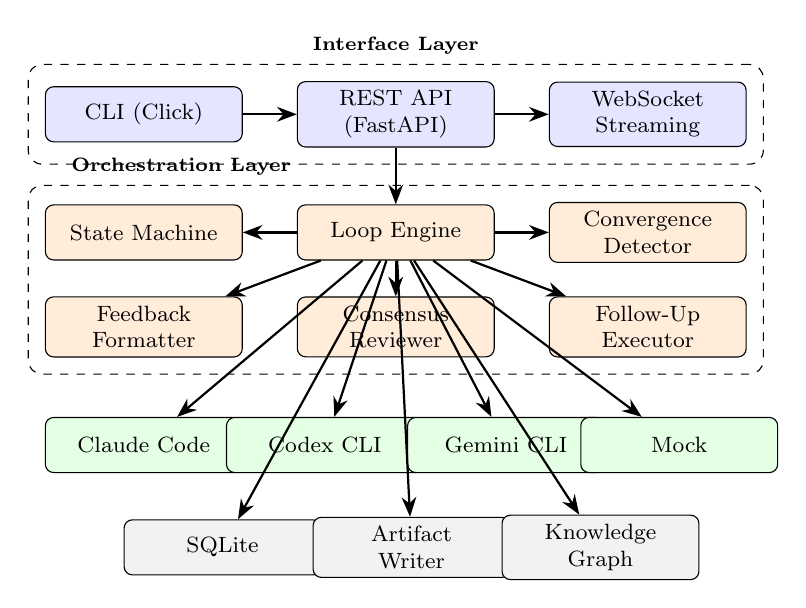
\begin{tikzpicture}[
  box/.style={rectangle, draw, rounded corners=3pt, minimum width=2.5cm, minimum height=0.7cm, align=center, font=\footnotesize},
  bigbox/.style={rectangle, draw, dashed, rounded corners=5pt, inner sep=6pt, align=center},
  arrow/.style={-{Stealth[length=2.5mm]}, thick},
  every node/.style={font=\footnotesize}
]

% CLI / API layer
\node[box, fill=blue!10] (cli) at (0, 5.2) {CLI (Click)};
\node[box, fill=blue!10] (api) at (3.2, 5.2) {REST API\\(FastAPI)};
\node[box, fill=blue!10] (ws) at (6.4, 5.2) {WebSocket\\Streaming};

% Engine layer
\node[box, fill=orange!15] (engine) at (3.2, 3.7) {Loop Engine};
\node[box, fill=orange!15] (sm) at (0, 3.7) {State Machine};
\node[box, fill=orange!15] (conv) at (6.4, 3.7) {Convergence\\Detector};
\node[box, fill=orange!15] (fb) at (0, 2.5) {Feedback\\Formatter};
\node[box, fill=orange!15] (cons) at (3.2, 2.5) {Consensus\\Reviewer};
\node[box, fill=orange!15] (fu) at (6.4, 2.5) {Follow-Up\\Executor};

% Adapter layer
\node[box, fill=green!10] (claude) at (0, 1.0) {Claude Code};
\node[box, fill=green!10] (codex) at (2.3, 1.0) {Codex CLI};
\node[box, fill=green!10] (gemini) at (4.6, 1.0) {Gemini CLI};
\node[box, fill=green!10] (mock) at (6.8, 1.0) {Mock};

% Persistence layer
\node[box, fill=gray!10] (db) at (1.0, -0.3) {SQLite};
\node[box, fill=gray!10] (artifacts) at (3.4, -0.3) {Artifact\\Writer};
\node[box, fill=gray!10] (knowledge) at (5.8, -0.3) {Knowledge\\Graph};

% Grouping boxes
\node[bigbox, fit=(cli)(api)(ws), label={[font=\scriptsize\bfseries]above:Interface Layer}] {};
\node[bigbox, fit=(engine)(sm)(conv)(fb)(cons)(fu), label={[font=\scriptsize\bfseries]above left:Orchestration Layer}] {};

% Arrows
\draw[arrow] (cli) -- (api);
\draw[arrow] (api) -- (engine);
\draw[arrow] (api) -- (ws);
\draw[arrow] (engine) -- (sm);
\draw[arrow] (engine) -- (conv);
\draw[arrow] (engine) -- (fb);
\draw[arrow] (engine) -- (cons);
\draw[arrow] (engine) -- (fu);
\draw[arrow] (engine) -- (claude);
\draw[arrow] (engine) -- (codex);
\draw[arrow] (engine) -- (gemini);
\draw[arrow] (engine) -- (mock);
\draw[arrow] (engine) -- (db);
\draw[arrow] (engine) -- (artifacts);
\draw[arrow] (engine) -- (knowledge);

\end{tikzpicture}
\caption{MI-Workbench architecture. The system comprises four layers: an interface layer (CLI, REST API, WebSocket), an orchestration layer (loop engine with state machine, convergence detection, feedback formatting, consensus review, and follow-up generation), a provider-agnostic adapter layer, and a persistence layer.}
\label{fig:architecture}
\end{figure}

\subsection{Workspace Model}
A \emph{workspace} represents an isolated research context with its own configuration, provider settings, budget limits, and git integration mode. Each workspace contains one or more \emph{runs}, where each run executes a loop definition against a specific research task. Runs produce versioned \emph{artifacts} organized by iteration: mechanistic analysis (\texttt{MECH.md}), evaluation reports (\texttt{EVAL.md}), experimental protocols (\texttt{XP.md}), methodology documentation (\texttt{METHOD.md}), and knowledge summaries (\texttt{KNOWLEDGE.md}).

\subsection{Data Model}
The system uses Pydantic~\citep{pydantic} for all data validation and serialization. Key models include \texttt{RunState} (tracking run lifecycle, iterations, token usage, and cost), \texttt{IterationResult} (individual step outcomes with artifacts and feedback), \texttt{ReviewResult} (structured critique with severity levels and artifact references), and \texttt{LoopDefinition} (graph-based workflow specification).

% ── 4. Workflow DSL ───────────────────────────────────────────────

\section{Graph-Based Workflow DSL}
\label{sec:dsl}

MI-Workbench defines research workflows as directed graphs where nodes represent agent roles and edges encode execution flow with conditions.

\subsection{Loop Definition}
A loop definition consists of \emph{nodes} and \emph{edges} specified in YAML:

\begin{lstlisting}[caption={Excerpt from the \texttt{executor\_reviewer} loop definition.}]
nodes:
  - id: executor
    role: executor
    prompt_ref: "executor/mi_executor"
  - id: reviewer
    role: reviewer
    prompt_ref: "reviewer/mi_reviewer"
  - id: adversarial
    role: adversarial_reviewer
    prompt_ref: "adversarial_reviewer/adversarial_reviewer"
edges:
  - source: executor
    target: reviewer
    condition: "always"
  - source: reviewer
    target: executor
    condition: "always"
  - source: reviewer
    target: adversarial
    condition: "every_k:3"
\end{lstlisting}

\subsection{Edge Conditions}
Three condition types are supported:
\begin{itemize}
  \item \texttt{always}: The edge is traversed every iteration.
  \item \texttt{every\_k:$N$}: The edge is traversed every $N$-th iteration (e.g., adversarial review every 3rd cycle).
  \item \texttt{on\_flag:$F$}: The edge is traversed only when flag $F$ is set (e.g., \texttt{on\_flag:high\_risk\_claims}).
\end{itemize}

\subsection{Compilation}
The DSL compiler performs a topological walk of the graph, validates structural integrity (no unreachable nodes, no duplicate IDs), and produces an ordered \texttt{ExecutionPlan} with a cycle length for infinite-loop repetition. Stop conditions include budget limits (tokens, cost, iterations), convergence detection, grade thresholds, and user-initiated cancellation.

\subsection{Built-in Presets}
Four presets are provided:
\begin{enumerate}
  \item \textbf{executor\_reviewer}: Standard executor--reviewer loop with periodic adversarial review.
  \item \textbf{reviewer\_consensus}: Three parallel reviewers (standard, adversarial, biological plausibility) with consensus merger.
  \item \textbf{research\_followups}: Executor--reviewer loop with automated follow-up proposal generation and optional auto-dispatch.
  \item \textbf{example\_custom}: Advanced loop with conditional adversarial escalation, knowledge extraction, and graph stability detection.
\end{enumerate}

% ── 5. Multi-Agent Orchestration ──────────────────────────────────

\section{Multi-Agent Orchestration}
\label{sec:orchestration}

\subsection{Agent Roles}

MI-Workbench defines nine specialized agent roles, each with a domain-specific system prompt:

\begin{table}[t]
\centering
\small
\caption{Agent roles and their research functions.}
\label{tab:roles}
\begin{tabular}{@{}lp{7.5cm}@{}}
\toprule
\textbf{Role} & \textbf{Function} \\
\midrule
Executor & Performs MI analysis: attention extraction, ablation studies, activation patching; produces MECH.md, XP.md, METHOD.md \\
Reviewer & Critiques claim validity, reproducibility, confounders, negative controls, and biological plausibility; produces EVAL.md \\
Adversarial Reviewer & Red-teams for p-hacking, overclaiming, causal confusion, dataset leakage, and statistical theater \\
Bio-Plausibility & Validates tissue specificity, pathway consistency, expression level plausibility, and regulatory direction \\
Idea Generator & Produces prioritized follow-up proposals with scientific value, feasibility, and novelty scores \\
Knowledge Extractor & Mines claims, estimates uncertainty, generates falsification tests \\
Automator & Designs reusable analysis pipelines from validated protocols \\
Publication Manager & Structures findings for manuscript preparation \\
Article Publisher & Formats results for communication \\
\bottomrule
\end{tabular}
\end{table}

\subsection{Execution Loop}
\label{sec:loop}

The core execution loop (Algorithm~\ref{alg:loop}) drives the iterative research process.

\begin{algorithm}[t]
\caption{MI-Workbench Execution Loop}
\label{alg:loop}
\begin{algorithmic}[1]
\REQUIRE RunState $R$, LoopDefinition $L$, Adapter $A$
\STATE $P \leftarrow \textsc{Compile}(L)$ \COMMENT{Compile to execution plan}
\STATE $i \leftarrow 0$, $\text{feedback} \leftarrow \emptyset$
\WHILE{$\neg\textsc{BudgetExceeded}(R) \wedge \neg\textsc{Converged}(R) \wedge \neg\textsc{Cancelled}(R)$}
  \STATE $s \leftarrow P.\text{steps}[i \bmod |P|]$
  \IF{$\neg\textsc{ShouldRun}(s, R.\text{iteration})$}
    \STATE $i \leftarrow i + 1$; \textbf{continue}
  \ENDIF
  \STATE $\text{prompt} \leftarrow \textsc{BuildPrompt}(s, R, \text{feedback})$
  \STATE $\text{result} \leftarrow \textsc{RunWithRetry}(A, \text{prompt})$
  \STATE $\text{result.output} \leftarrow \textsc{StripTraces}(\text{result.output})$
  \STATE $\text{artifacts} \leftarrow \textsc{ParseArtifacts}(\text{result.output}, s.\text{role})$
  \STATE $\textsc{WriteArtifacts}(\text{artifacts}, R.\text{iteration})$
  \IF{$s.\text{role} \in \{\text{reviewer}, \text{adversarial}\}$}
    \STATE $\text{review} \leftarrow \textsc{ParseReview}(\text{result.output})$
    \STATE $\text{feedback} \leftarrow \textsc{FormatFeedback}(\text{review})$
  \ELSE
    \STATE $\text{feedback} \leftarrow \text{result.output}$
  \ENDIF
  \STATE $\textsc{RecordConvergence}(R.\text{iteration}, \text{result})$
  \STATE $R.\text{iteration} \leftarrow R.\text{iteration} + 1$; $i \leftarrow i + 1$
\ENDWHILE
\RETURN $R$
\end{algorithmic}
\end{algorithm}

\subsection{State Machine}
Run lifecycle is managed by a finite state machine with states \{\textsc{Pending}, \textsc{Running}, \textsc{Paused}, \textsc{Stopped}, \textsc{Completed}, \textsc{Failed}\} and well-defined transitions. Paused runs can be resumed with full state reconstruction from the database and artifact filesystem. A crash recovery module detects interrupted runs on server restart, transitioning \textsc{Running} states with existing iterations to \textsc{Paused} for resumability.

\subsection{Convergence Detection}
Three convergence signals are monitored:
\begin{enumerate}
  \item \textbf{Grade stability}: The reviewer grade has remained constant for $w$ consecutive iterations (default $w{=}4$).
  \item \textbf{Zero critical issues}: No \textsc{Critical} or \textsc{High} severity critiques for $w$ iterations.
  \item \textbf{Output similarity}: Jaccard word-level similarity between consecutive executor outputs exceeds threshold $\tau$ for $w$ iterations.
\end{enumerate}
Any single signal triggers loop termination, preventing waste of compute on converged analyses.

\subsection{Retry Logic}
Adapter calls are wrapped in exponential backoff retry with jitter. Transient errors (rate limits, timeouts, connection failures) trigger retry with delay $d_k = d_0 \cdot 2^k \cdot (1 + \epsilon)$, where $\epsilon \sim \mathcal{U}(-0.25, 0.25)$. Permanent errors (authentication failures, invalid requests) fail immediately.

% ── 6. Consensus Review ──────────────────────────────────────────

\section{Consensus Review Mechanism}
\label{sec:consensus}

A central innovation of MI-Workbench is the \emph{consensus reviewer}, which addresses the limitations of single-reviewer assessment.

\subsection{Architecture}
The consensus reviewer runs three independent critic agents in parallel:
\begin{itemize}
  \item A \textbf{standard reviewer} evaluating claim validity, statistical rigor, and reproducibility.
  \item An \textbf{adversarial reviewer} specifically attacking for p-hacking, overclaiming, causal confusion, dataset leakage, biological implausibility, statistical theater, and null model inadequacy.
  \item A \textbf{biological plausibility checker} validating tissue specificity, pathway consistency, and expression level plausibility.
\end{itemize}

\subsection{Critique Merging}
\label{sec:merge}

The merging algorithm operates in four phases:

\paragraph{Phase 1: Parsing.}
Each reviewer's free-text output is parsed into structured \texttt{ReviewCritique} objects using multi-format detection: bracket format (\texttt{[SEVERITY] description}), Markdown format (\texttt{**Severity: X** --- description}), and structured format (\texttt{Severity: X, Category: Y, Description: Z}).

\paragraph{Phase 2: Deduplication.}
Critiques are grouped by Jaccard word-overlap similarity:
\begin{equation}
J(c_i, c_j) = \frac{|\text{words}(c_i) \cap \text{words}(c_j)|}{|\text{words}(c_i) \cup \text{words}(c_j)|}
\end{equation}
Pairs with $J(c_i, c_j) \geq \tau$ (default $\tau{=}0.5$) are merged into a single group.

\paragraph{Phase 3: Severity escalation.}
Within each group, the maximum severity is selected. If two or more reviewers independently flagged the same issue, severity is escalated by one level (capped at \textsc{Critical}). This implements the intuition that inter-reviewer agreement signals higher importance.

\paragraph{Phase 4: Ranking.}
Merged critiques are sorted by severity (descending), then by number of contributing reviewers (descending), producing a prioritized list for the executor.

\subsection{Grade Computation}
An overall grade is computed from the merged critique list: $\geq 2$ \textsc{Critical} issues $\Rightarrow$ F; $\geq 1$ \textsc{Critical} $\Rightarrow$ D; $\geq 3$ \textsc{High} $\Rightarrow$ D; $\geq 1$ \textsc{High} $\Rightarrow$ C; $\geq 1$ \textsc{Medium} $\Rightarrow$ B; otherwise A.

% ── 7. Structured Feedback ───────────────────────────────────────

\section{Structured Feedback and Output Cleaning}
\label{sec:feedback}

\subsection{Artifact-Aware Feedback}

A key finding from initial deployments was that generic feedback (``Previous iteration output: \ldots Continue with: task'') produced shallow revisions. We introduced \emph{artifact-aware feedback} with two innovations:

\paragraph{Reference inference.}
When parsing reviewer critiques, the system infers artifact references (e.g., \texttt{PROTOCOL.md}) and section references (e.g., ``Section 2.1 Controls'') from the critique text using pattern matching against known artifact names and section header patterns. These references are attached to each \texttt{ReviewCritique} as \texttt{artifact\_ref} and \texttt{section\_ref} fields.

\paragraph{Revision framing.}
Instead of the generic ``Continue with: task'' prompt, revision iterations use structured framing:

\begin{lstlisting}[caption={Revision prompt template injected for post-review iterations.}]
=== REVISION REQUEST (Iteration N) ===
You produced artifacts in the previous iteration.
The reviewer has identified specific issues.

=== REVIEWER FEEDBACK (Grade: B) ===
REQUIRED FIXES (must address):
1. [CRITICAL | stats | EVAL.md Section 3.2]
   p-value without effect size
2. [HIGH | reproducibility | PROTOCOL.md Section 2.1]
   Missing dataset URLs
SUGGESTED IMPROVEMENTS:
3. [MEDIUM | general] Consider cell-type decomposition
=== END FEEDBACK ===

TASK: Revise your artifacts to address ALL required
fixes above. Make targeted revisions, not rewrites.
\end{lstlisting}

\subsection{Output Cleaning Pipeline}

LLM outputs frequently contain ``thinking traces''---narration about the model's intended actions (e.g., ``I will read the file\ldots'', ``Let me check the data\ldots'') that contaminate research artifacts. The output cleaning module removes these traces using regex-based line filtering:

\begin{itemize}
  \item Forward-looking narration: ``I will\ldots'', ``I'll\ldots'', ``Let me\ldots''
  \item Tool-call narration: ``I will read/search/check the\ldots''
  \item Sequencing prefixes: ``First, I will\ldots'', ``Next, I'll\ldots''
  \item Meta-commentary: ``The following is\ldots''
\end{itemize}

The cleaner preserves code blocks (tracking \texttt{```} fences), markdown headers, and substantive past-tense narration. Cleaning is applied immediately after adapter output, before any downstream consumer (artifact parser, feedback formatter, consensus merger).

% ── 8. Provider-Agnostic Adapter Layer ───────────────────────────

\section{Provider-Agnostic Adapter Layer}
\label{sec:adapters}

MI-Workbench defines a \texttt{BaseAdapter} abstract interface with three methods: \texttt{run(request) $\to$ result}, \texttt{smoke\_test() $\to$ status}, and \texttt{is\_available() $\to$ bool}. Four implementations are provided:

\begin{table}[t]
\centering
\small
\caption{Adapter implementations and their CLI invocation patterns.}
\label{tab:adapters}
\begin{tabular}{@{}llp{4.8cm}@{}}
\toprule
\textbf{Adapter} & \textbf{Binary} & \textbf{Invocation} \\
\midrule
Claude Code & \texttt{claude} & \texttt{claude -p --output-format json --max-turns 1 --system-prompt \$SP} \\
Codex CLI & \texttt{codex} & \texttt{codex exec --full-auto --skip-git-repo-check -} \\
Gemini CLI & \texttt{gemini} & \texttt{gemini --yolo -p \$PROMPT} \\
Mock & --- & Synthetic role-aware responses with configurable grade progression \\
\bottomrule
\end{tabular}
\end{table}

The mock adapter produces realistic MI research outputs with role detection from prompt content, grade progression (C $\to$ B $\to$ B$+$ $\to$ A$-$), and synthetic metrics (AUROC, correlation, validation splits) with diminishing variation across iterations. This enables rapid prototyping and comprehensive testing without LLM API costs.

% ── 9. Knowledge Extraction ──────────────────────────────────────

\section{Knowledge Extraction and Claim Management}
\label{sec:knowledge}

MI-Workbench includes a knowledge extraction pipeline that mines structured claims from research artifacts.

\subsection{Claim Detection and Classification}
Claims are detected via pattern matching on phrases such as ``we found that\ldots'', ``results show\ldots'', ``AUROC = X'', and ``$p < 0.05$''. Detected claims are classified as \emph{empirical}, \emph{methodological}, \emph{interpretive}, or \emph{comparative}.

\subsection{Uncertainty Estimation}
Each claim receives an uncertainty score $u \in [0, 1]$ (baseline 0.5) adjusted by: strong evidence ($p < 0.001$): $u \leftarrow u - 0.2$; confidence intervals present: $u \leftarrow u - 0.1$; hedging language (``suggests'', ``may''): $u \leftarrow u + 0.1$; large sample ($n \geq 1000$): $u \leftarrow u - 0.1$.

\subsection{Falsification Test Generation}
For each claim type, the system auto-generates falsification suggestions: AUROC claims prompt stronger baselines (mutual information, variance-based features); layer-specific claims prompt split-sample validation; attention claims prompt residualization tests; statistical claims prompt stringent multiple testing correction.

\subsection{Claim Graph}
Claims are stored in a relational database with support for inter-claim relationships (supports, contradicts, extends) and evidence linking. A graph API enables visualization of the claim network, supporting identification of weakly-supported claims and contradictions.

% ── 10. Reproducibility ──────────────────────────────────────────

\section{Reproducibility Infrastructure}
\label{sec:reproducibility}

\subsection{Artifact Versioning}
Each iteration writes artifacts to a structured directory: \texttt{workspace/runs/\{run\_id\}/iter\_NNNN/MECH.md}. This provides full provenance: every revision of every artifact is preserved with its iteration context.

\subsection{Git Integration}
Four git modes are supported: \texttt{none} (no version control), \texttt{commit\_per\_run} (single commit after run completion), \texttt{commit\_per\_iteration} (commit after each iteration), and \texttt{branch\_per\_run} (create a dedicated branch \texttt{run/\{run\_id\}}).

\subsection{Reproducibility Packages}
The \texttt{repropack} generator creates self-contained ZIP archives containing: all artifacts organized by iteration, \texttt{run\_meta.json} with run configuration and timing, \texttt{prompts\_used.json} with resolved prompt templates, \texttt{environment.json} with Python version and installed packages, \texttt{git\_state.json} with branch and commit hash, and auto-generated dataset cards and reproducibility checklists.

% ── 11. Case Study ───────────────────────────────────────────────

\section{Case Study: Geneformer Attention and Causal Regulation}
\label{sec:casestudy}

We validated MI-Workbench on a substantive MI question: \emph{Do attention heads in Geneformer encode causal gene regulatory relationships, or do they merely reflect co-expression patterns?}

\subsection{Experimental Setup}
We used the Gemini CLI adapter to run 11 end-to-end experiments across three loop presets:

\begin{table}[t]
\centering
\small
\caption{Case study runs. All runs used the Gemini CLI adapter.}
\label{tab:runs}
\begin{tabular}{@{}clcc@{}}
\toprule
\textbf{Run} & \textbf{Preset} & \textbf{Iters.} & \textbf{Task Summary} \\
\midrule
1--3 & executor\_reviewer & 1 & AUROC interpretation, encoding, ablation \\
4 & executor\_reviewer & 5 & Experimental protocol design \\
5 & research\_followups & 3 & Paradox analysis (23$\times$ logit perturb.) \\
6 & reviewer\_consensus & 3 & Non-K562 generalization critique \\
7 & executor\_reviewer & 4 & Methods comparison document \\
8 & executor\_reviewer & 3 & Attention--co-expression (validation) \\
\bottomrule
\end{tabular}
\end{table}

\subsection{Key Findings from Automated Analysis}

The platform autonomously identified three primary confounders explaining the attention--co-expression correlation:

\paragraph{MLM Objective Confounder.}
The executor agent correctly identified that Geneformer's masked language modeling objective incentivizes attending to co-expression cliques rather than causal regulators, because co-expressed genes are the most statistically powerful predictors of masked token identity.

\paragraph{Rank-Value Encoding Artifacts.}
The system identified that Geneformer's rank-value tokenization creates an inductive bias where positional proximity in the sequence corresponds to expression magnitude similarity, producing false-positive attention between co-abundant genes rather than regulatory links.

\paragraph{Attention Symmetry.}
Standard dot-product attention $\text{softmax}(QK^\top)$ is inherently bidirectional unless the model learns distinct query/key projections. The executor noted that $A_{ij} \approx A_{ji}$ fails to capture the directional nature of gene regulation (TF $\to$ Target).

\subsection{Iterative Refinement Quality}

The structured feedback mechanism produced measurable quality improvements across iterations:

\begin{itemize}
  \item \textbf{Iteration 1} (executor): Initial analysis with three confounders, protocol outline with null hypotheses.
  \item \textbf{Iteration 2} (reviewer): Identified missing controls---cell-type composition confounder, unspecified dataset, missing BH-FDR correction details.
  \item \textbf{Iteration 3} (executor revision): Added within-cluster partial correlation control, specified Genecorpus-30M bone marrow subset, defined mean rank baseline, and set random seed.
\end{itemize}

Critically, the revision iteration produced \emph{targeted changes} to the specific artifacts and sections referenced in the feedback, rather than rewriting from scratch---a direct result of the artifact-aware feedback mechanism.

\subsection{Output Quality Assessment}

Post-hoc validation by domain experts confirmed:
\begin{itemize}
  \item All three identified confounders are well-documented in the literature~\citep{pratapa2020benchmarking,theodoris2023transfer}.
  \item The proposed null hypotheses ($H_0^1$: co-expression dominance, $H_0^2$: attention symmetry, $H_0^3$: degree bias) are scientifically appropriate.
  \item Statistical framework choices (AUPRC over AUROC for sparse networks, BH-FDR correction) reflect current best practices.
  \item The output contained no ``thinking traces'' (validated by comparison with pre-cleaning runs where traces contaminated all artifact files).
\end{itemize}

% ── 12. Implementation ───────────────────────────────────────────

\section{Implementation}
\label{sec:implementation}

MI-Workbench is implemented in Python 3.11 using FastAPI for the REST API, aiosqlite for async database operations, Click for the CLI, and Pydantic for data validation.

\begin{table}[t]
\centering
\small
\caption{Codebase statistics.}
\label{tab:stats}
\begin{tabular}{@{}lr@{}}
\toprule
\textbf{Metric} & \textbf{Value} \\
\midrule
Backend source files & 40+ \\
Test files & 26 \\
Total test functions & 360 \\
Loop preset definitions & 4 \\
Prompt templates & 9 \\
API endpoints & 25+ \\
Supported providers & 4 \\
Database tables & 7 \\
\bottomrule
\end{tabular}
\end{table}

Key implementation decisions include:
\begin{itemize}
  \item \textbf{Async throughout}: All I/O operations (database, adapter calls, file writes) use \texttt{async}/\texttt{await} for concurrency.
  \item \textbf{SQLite with WAL mode}: Write-Ahead Logging enables concurrent reads during long-running writes, validated under stress testing with 10 concurrent runs.
  \item \textbf{Event-driven architecture}: The engine emits events (\texttt{iteration\_started}, \texttt{iteration\_completed}, etc.) broadcast to WebSocket clients for real-time monitoring.
  \item \textbf{Crash recovery}: On server restart, interrupted runs are detected and transitioned to resumable states.
\end{itemize}

% ── 13. Discussion ───────────────────────────────────────────────

\section{Discussion}
\label{sec:discussion}

\paragraph{Strengths.}
MI-Workbench demonstrates that multi-agent orchestration can produce research-quality MI analyses without human intervention. The consensus reviewer mechanism provides robustness against individual agent blind spots. The provider-agnostic design insulates research workflows from vendor lock-in. The comprehensive test suite (360 tests including stress tests and fuzzing) provides confidence in system reliability.

\paragraph{Limitations.}
Several limitations warrant discussion:
\begin{enumerate}
  \item \textbf{No code execution}: The current system generates analysis \emph{plans} and \emph{protocols} but does not execute computational code. Integrating sandboxed code execution (e.g., via Jupyter kernels) would enable fully autonomous experimental pipelines.
  \item \textbf{Convergence detection granularity}: The current Jaccard-based similarity metric is coarse. Semantic similarity via embeddings could provide finer-grained convergence signals.
  \item \textbf{Cost tracking}: Token usage and cost estimation depend on adapter-level reporting, which varies by provider. Standardized cost accounting across providers remains an open challenge.
  \item \textbf{Human-in-the-loop}: While the system supports the \texttt{ask\_approval} policy for follow-ups, there is no mechanism for mid-loop human intervention to redirect analyses.
\end{enumerate}

\subsubsection*{Broader Impact Statement}
The automation of research critique raises questions about the appropriate level of human oversight. We advocate for MI-Workbench as an \emph{augmentation} tool that accelerates the hypothesis--critique cycle, not as a replacement for expert judgment. The reproducibility packaging ensures that all automated analyses can be scrutinized by human reviewers. We note that the system's domain-specific prompts encode assumptions about statistical best practices and biological plausibility that reflect current community consensus; these assumptions should be periodically reviewed as norms evolve.

% ── 14. Conclusion ────────────────────────────────────────────────

\section{Conclusion}
\label{sec:conclusion}

We presented MI-Workbench, an open-source platform for autonomous multi-agent mechanistic interpretability research. The system's graph-based workflow DSL, consensus review mechanism, structured feedback injection, and provider-agnostic architecture enable rigorous, reproducible MI investigations. Validation on the Geneformer attention--regulation question demonstrates that the platform can autonomously identify confounders, propose controlled experiments, and iteratively refine analyses to research-grade quality. MI-Workbench provides a foundation for scaling mechanistic interpretability of biological foundation models beyond the capacity of individual researchers. Code and documentation are available at \url{https://github.com/Biodyn-AI/mi-workbench}.

\bibliography{references}
\bibliographystyle{tmlr}

\appendix
\section{Appendix: Future Directions}
\label{app:future}

Key extensions include: (i) sandboxed code execution for computational experiments; (ii) integration with lab automation systems for wet-lab validation; (iii) multi-model ensemble execution (running the same task across multiple LLMs and comparing outputs); (iv) active learning for convergence thresholds; and (v) formal verification of statistical claims via symbolic computation.

\end{document}
